\chapter{Belle~\RN{2}}
\label{chap:belle2_experiment}

\section{Experiment}
\label{sec:experimental}

The Belle~\RN{2} experiment is performed at the SuperKEKB accelerator located in Tsukuba, Ibaraki Prefecture, Japan. It is designed to study the B meson.
In the experiment, asymmetric electron- positron-beams are collided with a center of mass energy of $\sqrt{s} = 10.58 \mathrm{~GeV}$, just right to create the $\Upsilon (4S)$ meson. The two beams, positrons at $4 \mathrm{~GeV}$ and electrons at $7 \mathrm{~GeV}$, are focussed to a narrow but slightly elliptical crossing section. The non-circular shape is due to the angle between both beams. The additional boost in one direction is used to measure the B-lifetime.

In comparison to the predecessor experiment Belle, the integrated luminosity will be $50$ times higher at $50~{ab}^{-1}$ while the instantaneous luminosity will be increased $40$-fold to $8 \cdot 10^{35} \mathrm{cm}^{-2} \mathrm{s}^{-1}$.

\section{Detector system}
\label{sec:detector_system}

\subsection{Overview}
\label{subsec:detector_system_overview}

This part mainly relies on the Belle~\RN{2} Technical Design Report~\cite{Abe:2010gxa} and the secondary sources~\cite{Pulvermacher:SuperKEKBDetectorComponents} and~\cite{Pulvermacher:AnalysisSoftware}. Additionally, if not specifically stated, otherwise the charge conjugate of a particle is implied.

The Belle~\RN{2} detector system is a composition of multiple detectors, each measuring a subset of properties of a particle's track.
The inner three detectors --- \textbf{P}i\textbf{X}el \textbf{D}etector (PXD), \textbf{S}ilicon \textbf{V}ertex \textbf{D}etector (SVD) and \textbf{C}entral \textbf{D}rift \textbf{C}hamber (CDC) --- record the position of particles. Hence they are also called tracking detectors. They are located in a homogeneous magnetic field of $1.5~\mathrm{T}$.
The innermost detector is the PXD. Together with the SVD which is located right after the PXD, it is used to reconstruct decay vertices and identify tracks belonging to particles with a low-momentum.
The CDC measures the momentum and charge of particles via their curvature in the magnetic field.
Next, the \textbf{T}ime \textbf{O}f \textbf{P}ropagation counter (TOP) (`Barrel PID' in \autoref{fig:belle2_detector_design_white_paper}) and the \textbf{A}erogel \textbf{R}ing-\textbf{I}maging \textbf{CH}erenkov (ARICH) counter (`Endcap PID' in \autoref{fig:belle2_detector_design_white_paper}) are used to identify charged particles via their emission of Cherenkov radiation in the detector. However, there is no such installation for the backwards-facing endcap of the detector.
The \textbf{E}lectromagnetic \textbf{C}a\textbf{L}orimeter (ECL) identifies photons and electron.
The outermost detector called $\boldsymbol{K}^0_{\boldsymbol{L}}$/$\boldsymbol{\mu}$ (KLM) is used to identify kaons and muons.

\begin{figure}[ht]
	\centering
	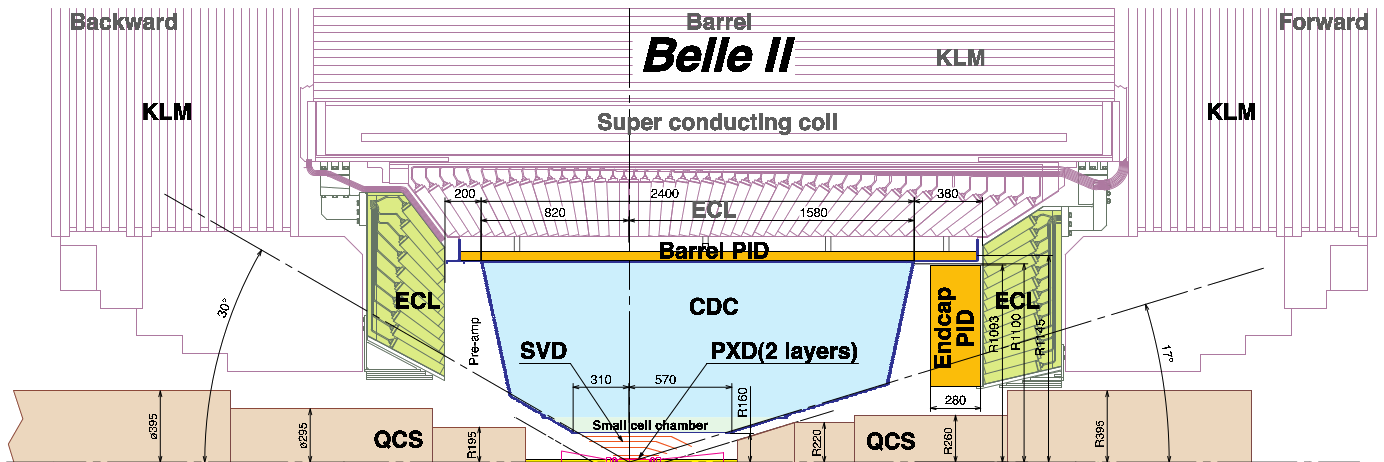
\includegraphics[width=\textwidth,height=0.6\textheight,keepaspectratio]{{{../res/Belle 2 detector design white paper (truncated)}}}
	\caption{Side view of the upper half of the Belle~\RN{2} detector. The bottom half (not shown in the picture) would correspond to the mirror image alongside the beampipe. Adapted from~\cite{Abe:2010gxa}.}
	\label{fig:belle2_detector_design_white_paper}
\end{figure}

\subsection{Silicon detectors}
\label{subsec:detector_system_silicon_detectors}

The PXD and SVD consist of tiny doped silicon chips which yield the location of electron-holes created by particles passing through it. The PXD detector uses small pixels while the SVD detector uses strips of detector materials. Therefore the PXD detector is able to further differentiate multiple simultaneous tracks while the SVD allows for a faster readout and is less prone to noise.

\subsection{Central drift chamber}
\label{subsec:detector_system_tracking_detectors}

The CDC, which surrounds the PXD and SVD, consists of a collection of charged wires and detection wires located volume filled with gas. The detection wires are used to measure the current produced by electromagnetic showers. The latter is caused by particles passing through the gas. The wires are close to being parallel to the beampipe but have a slight twist. This allows the detector to not only have an excellent estimation of the transverse distance to the beam pipe but also provides information about the longitudinal position.

\subsection{Barrel and endcap PID}
\label{subsec:detector_system_barrel_and_endcap_pid}

The Cherenkov effect is used to measure the velocity of particles in the TOP and ARICH detector. Charged particles which travel faster than the speed of light in the medium --- Quartz in case of the TOP detector and aerogel for the ARICH detector --- produce light due to their uneven polarization of the medium. The velocity can be calculated by measuring the time of propagation and the angle of the emitted light (Cherenkov angle).

\subsection{Electromagnetic calorimeter}
\label{subsec:detector_system_electromagnetic_calorimeter}

The main purpose of the ECL detector is to measure the position and energy of photons and electrons. Both particle species excite the medium and create electromagnetic showers. The light of the de-excitation can subsequently be measured.

\subsection{$\boldsymbol{K}^0_{\boldsymbol{L}}$/$\boldsymbol{\mu}$ detector}
\label{subsec:detector_system_k0lmu}

Last but not least the KLM detector measures the penetration ability of particles in order to differentiate between muons and kaons. When flying through the detector, the particles pass through plates serving as electrodes separated by a layers of gas in between them. Ionized particles are accelerated in this field and subsequently produce a spark picked up by the detector via measuring the drop in voltage.

\section{Interaction with matter}
\label{sec:interaction_with_matter}

\subsection{Charged particle interaction}
\label{subsec:interaction_with_matter}

Particles with a non-zero charge mainly interact with the medium electromagnetically. In general, an interaction occurs either by scattering in the electric field of the atom, polarization of the medium, ionization, excitation or scattering at the atom itself. Particles and their anti-particles additionally have the ability to annihilate.

The polarization of the medium causes Cherenkov radiation to be emitted. At velocities below the speed of light in the medium ($v < c/n$), nothing of interest may be observed. However, at $v > c/n$ the Cherenkov effect must be taken into account. The effect occurs due to the information about the charge of the traversing particle not reaching the medium in front of it soon enough. Hence, the medium behind the particle is already aligned with the electric field while the medium in front is not. The result is an electromagnetic wave. The angle between the normal vector of the wave and the track of the particle is given by
\begin{equation}
	\cos(\Theta_{c}) = \frac{1}{v/c \cdot n} = \frac{1}{\beta \cdot n}
	\mathrm{.}
\end{equation}
This is the effect upon which the TOP and ARICH detectors are built.

Particles with low energy traveling through a medium interact predominantly with atomic electrons. The average energy loss of a particle is described by the Bethe-Bloch formula. It is given by $\left< \mathrm{d}E/\mathrm{d}x \right> \propto 1/{\beta^2}$ for velocities of up to about $90\%$ of the speed of light and is minimal at $\beta \gamma \approx 4$. As such it describes the momentum dependency of the average energy loss. However, the actual shape of $\mathrm{d}E/\mathrm{d}x$ is modelled by the Landau distribution. Note that the initial assumptions needed for this formula are not met for electrons. This is because both parties of the interaction belong to the same species and have identical masses.
A $\mathrm{d}E/\mathrm{d}x$-measurement is performed at the silicon detectors and the CDC.

The interaction with the electromagnetic field of the nucleus is the dominant cause for the loss of energy for high-energy particles. Energy is radiated away via so called Bremsstrahlung. The leftover energy decreases exponentially with the distance traversed and is inversely proportional to the square root of the mass. Therefore it is most important for particles with a low mass, e.g., electrons. The radiation due to this effect is mainly measured by the ECL.

\subsection{Particle identification}
\label{subsec:particle_identification}

At Belle~\RN{2} the detector system differentiates among six long living particle species: $\{K, \pi, e, \mu, p, \hbox{deuteron}\}$.

The $\mathrm{d}E/\mathrm{d}x$-measurement from the silicon detectors and the CDC are one of the most useful yields. \autoref{fig:de_dx_for_SVD} showcases this for one of the tracking detectors for momentums below $1 \mathrm{~GeV/c}$. Distinct patterns may be observed for various particle species below this momentum threshold. The fact that the mean energy loss in the graph is truncated, denotes that in order to reduce outliers the lowest $5\%$ and highest $25\%$ of each track are not used in the estimation.
New tracks can now be assigned a likelihood of belonging to a particle species. This is done by putting forward a hypothesis for the loss of energy for each such species.

ARICH, TOP and CDC furthermore extend the identification and are able to differentiate among $\{K, \pi, p, \hbox{deuteron}\}$ rather reliably but also contribute to $\{e, \mu\}$. They provide likelihoods for each signal given a particle hypothesis as well.

Further out the ECL detector provides a good separation of electrons from other charged particles above $1 \mathrm{~GeV/c}$. It is able to do so via measuring $E/p$ of the shower. The detector response is provided by estimating the degree of agreement for different particle hypothesis with the signal. An exemplary $E/p$ curve is shown in \autoref{fig:e_p_for_ECL}. It demonstrates the observable difference for electrons compared to other particle species but also shows that no clear separation of pions and muons is possible.

The KLM detector provides a good separation between muons and non-muons and yields such separation in the form of different likelihoods as well.

\begin{figure}[ht]
	\centering
	\subcaptionbox{Truncated $\mathrm{d}E/\mathrm{d}x$ means as a function of momentum in the SVD with the color encoding the number of hits. Taken from~\cite{Belle2Collaboration:B2TiP}.\label{fig:de_dx_for_SVD}}{
		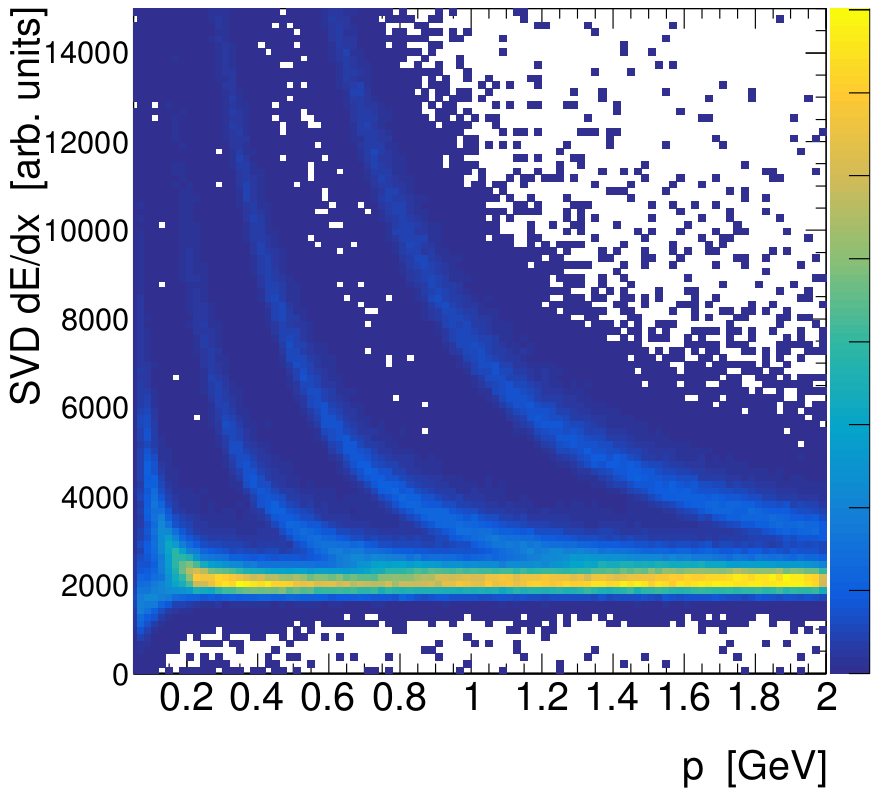
\includegraphics[width=0.43\textwidth,height=\textheight,keepaspectratio]{{{../res/dE dx for SVD detector by particles}}}
	}
	\hspace{2em}
	\subcaptionbox{$E/p$ distribution for different particle species. Taken from~\cite{Belle2Collaboration:B2TiP}.\label{fig:e_p_for_ECL}}{
		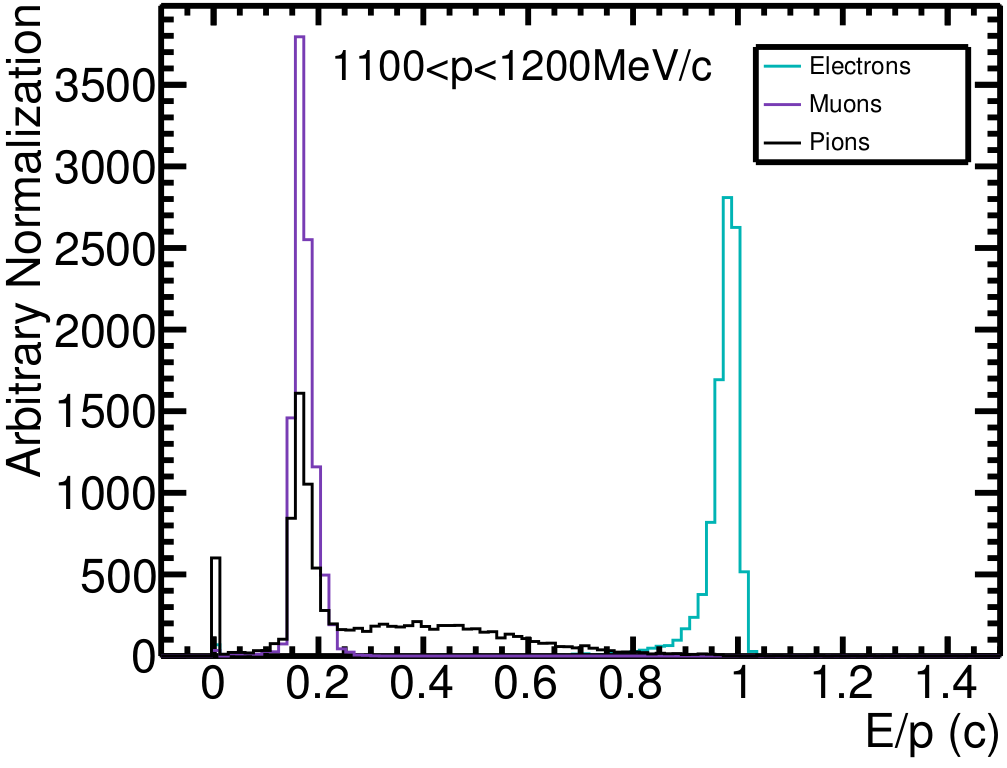
\includegraphics[width=0.43\textwidth,height=\textheight,keepaspectratio]{{{../res/E p for ECL detector by particles}}}
	}
	\caption{Separation of different particle species for various signals.}
\end{figure}

